%\documentclass[8pt, handout]{beamer}
%\usepackage{pgfpages} 								%Для распечатки
%\pgfpagesuselayout{2 on 1}[a4paper,border shrink=10mm]

\documentclass[8pt]{beamer}

\usepackage[english,russian]{babel}
\usepackage[utf8]{inputenc}
\usepackage{mflogo}
\usepackage{amsmath,amsfonts,amssymb}
\usepackage{euscript}
\usepackage{graphicx}
\usepackage{xcolor}
\usepackage{transparent}



\beamertemplatenavigationsymbolsempty

\usetheme{EastLansing}
\setbeamercovered{transparent}


\title[Интегральное исчисление]{Математический анализ\\ Тема 4: Интегральное исчисление}
\author[Выборный Е. В.]{Выборный Евгений Викторович\\ email: evybornyi@hse.ru}
\date{Москва 2016} 


\makeatletter
\setbeamertemplate{footline}{
    \leavevmode%
    \hbox{%
    \begin{beamercolorbox}[wd=.25\paperwidth, ht=2.5ex, dp=1ex, center]{author in head/foot}%
        \usebeamerfont{author in head/foot}%
        \insertshortauthor
    \end{beamercolorbox}%
    \begin{beamercolorbox}[wd=.5\paperwidth,ht=2.5ex,dp=1ex,center]{title in head/foot}%
        \usebeamerfont{title in head/foot}\insertshorttitle
    \end{beamercolorbox}%
    \begin{beamercolorbox}[wd=.25\paperwidth,ht=2.5ex,dp=1ex,right]{date in head/foot}%
        \usebeamerfont{date in head/foot}\insertshortdate{}\hspace*{2em}
        \insertframenumber{} / \inserttotalframenumber\hspace*{2ex}
    \end{beamercolorbox}}%
    \vskip0pt%
}
\makeatother

\makeatletter
\setbeamertemplate{title page}
{
\centering
 \usebeamerfont{author}\insertauthor
 \vfill
 \begin{beamercolorbox}[rounded=true,shadow=true,sep=8pt,center]{title}
  \usebeamerfont{title}\inserttitle
 \end{beamercolorbox}
\vfill
\centering
\insertdate\par
 \vskip0.2em
}
\makeatother

\begin{document}
%\parindent=1.5em %красная строка

\begin{frame}
\titlepage
\end{frame}

\begin{frame}{Первообразная}
На практике часто возникает задача по функции $f$, заданной на некотором промежутке, найти функцию $F$ такую, что производная $F$ совпадает с $f$:
$$F'(x) = f(x).$$
Например, если известна скорость движения материальной точки в различные моменты времени и необходимо определить пройденный путь.

\begin{block}{Определение. Первообразная}
Дифференцируемая функция $F(x)$ называется {\bf первообразной} (неопределенным интегралом) для функции $f(x)$ на заданном промежутке, если $F'(x)=f(x)$.
Используют обозначения:
$$F(x) = \int f(x)dx.$$
\end{block}
Таким образом, по определению:
$$\frac{d}{dx}\int f(x)dx = f(x),$$
для всех $x$ из заданного промежутка.
\end{frame}

\begin{frame}{Первообразная. Основная теорема}
При рассмотрении задачи поиска первообразной естественными являются вопросы о существование и единственности первообразной для заданной функции на определенном интервале.

\begin{block}{Теорема}
Если первообразная $F(x)$ для функции $f(x)$ существует, то любая функция вида $F(x) + C$, где $C$ --- константа, будет первообразной для $f(x)$ и обратно: любая первообразная $\Phi(x)$ функции $f(x)$ обязательно имеет такой вид, то есть
$$\Phi(x)=F(x)+A,$$
где $A$ --- определенная константа, для всех $x$ из рассматриваемого промежутка.
\end{block}

\begin{block}{Доказательство}
Первое утверждение очевидно, поскольку:
$$\left( F(x)+C \right)' = F'(x) = f(x).$$
Докажем, что разность двух первообразных --- величина постоянная. Действительно, $$\left(\Phi(x) - F(x) \right)' =\Phi'(x)  - F'(x) = f(x) - f(x) = 0.$$
Таким образом, второе утверждение теоремы следует из признака постоянства функции.
\end{block}

\end{frame}

\begin{frame}{Таблица первообразных}
Вопрос существования первообразной значительно сложнее и будет частично рассмотрен в дальнейшем. Отметим, что для любой непрерывной функции первообразная существует.
\vskip1em
Поскольку нам известны производные ряда базовых элементарных функций, можно составить таблицу неопределенных интегралов:
\begin{center}
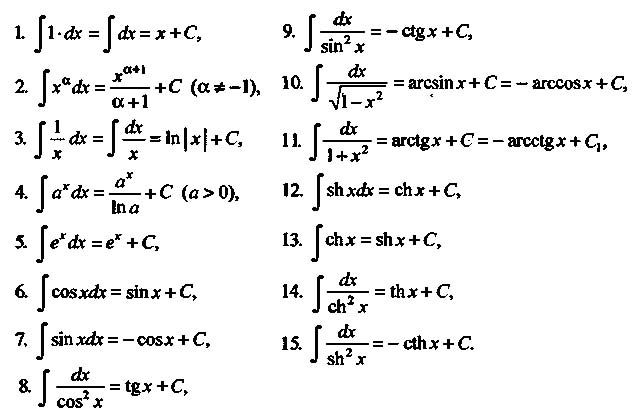
\includegraphics[scale=0.4]{Itable.jpg}
\end{center}
\end{frame}

\begin{frame}{Первообразная. Пример}
Рассмотрим подробнее случай $f(x)=1/x$. Функция $f(x)$ непрерывна при $x\ne 0$. Следовательно, необходимо отдельно рассмотреть промежутки $x>0$ и $x<0$.
\vskip1em
Пусть $x>0$. Тогда
$$\left( \ln(x) \right)' = \frac{1}{x} \quad \Rightarrow \quad \int \frac{dx}{x} = \ln(x) +c_1.$$
Пусть $x<0$. Тогда
$$\left( \ln(-x) \right)' = \frac{-1}{-x}=\frac{1}{x} \quad \Rightarrow \quad \int \frac{dx}{x} = \ln(-x) +c_2.$$
Оба этих случая можно записать вместе в следующем виде:
$$\int\frac{dx}{x} = \ln|x| + c.$$
Стоит отметить, что, если задача стоит в поиске общего вида первообразной $F(x)$ для функции $1/x$ при всех $x\ne 0$, то она имеет вид:
$$F(x)=\left\{
\begin{array}{ll}
\ln(x)+c_1& x>0;\\
\ln(-x)+c_2& x<0,
\end{array}\right.
$$
где $c_1$ и $c_2$ не обязательно совпадают.
\end{frame}

\begin{frame}{Свойства неопределенного интеграла}
Простейшие свойства неопределенного интеграла непосредственно следуют из соответствующих свойств дифференцирования.
\begin{block}{Линейность}
Интегрирование является линейной операцией:
$$\int (A\, f(x) + B\, g(x) ) dx = A \int f(x)dx + B \int g(x)dx.$$
\end{block}
\vskip-1em
\begin{block}{Доказательство}
Пусть $F$ и $G$ --- первообразные для функций $f$ и $g$ соответственно. Тогда
$$\left( A\, F(x) + B\, G(x) \right)' = A\, F'(x) + B\, G'(x) = A\, f(x) + B\, g(x).$$
Следовательно, $A\, F(x) + B\, G(x)$ --- первообразная для линейной комбинации  $A\, f(x) + B\, g(x) $, что и требовалось доказать.
\end{block}
\begin{block}{Пример}
$$\int\left(1+2x+5\sqrt{x}\right)dx =x+x^2+5\cdot\frac{2}{3}x^{3/2}+C.$$
\end{block}
\end{frame}

\begin{frame}{Свойства неопределенного интеграла}
\begin{block}{Замена переменных}
Из правила дифференцирования сложной функции следует правило замены переменной в неопределенном интеграле:
$$\int f(x) dx = \int f(x(t)) x'(t) dt ,$$
где $x=x(t)$ непрерывно дифференцируемая функция, имеющая обратную функцию $t=t(x)$.
\end{block}
Это правило применяют, если интеграл от функции $g(t) = f(x(t))x'(t)$ по переменной $t$ найти проще, чем исходный интеграл от $f(x)$ по $x$. Иногда это правило удобно записывать в виде:
$$\int f(x) dx = \int f(x(t)) dx(t),$$
поскольку $dx(t) = x'(t)dt$.
\begin{block}{Линейная замена}
В простейшем случае применяется линейная замена $a x+b=t(x)$. Тогда $dx=\frac{1}{a}dt$,
$$\int f(a x+b)dx =\frac{1}{a} \int f(t) dt.$$
\end{block}
\end{frame}

\begin{frame}{Примеры вычисления неопределенного интеграла}
\begin{block}{Примеры}
\begin{enumerate}
\item Вычислим интеграл:
$$\int e^{2x}dx =\left\{ 2x =t,\ dx=\frac{1}{2} dt \right\} = \frac{1}{2} \int e^{t}dt = \frac{1}{2}e^t+C = \frac{1}{2}e^{2x}+C.$$
Обычно линейные замены переменной в интеграле производится в уме.
\item Вычислим интеграл:
$$\int \frac{dx}{1-x^2}.$$
В данном случае удобно разложить дробь $1/(1-x^2)$ на две более простых дроби:
$$\frac{1}{1-x^2} = \frac{1}{2}\left( \frac{1}{1+x}+\frac{1}{1-x}\right).$$
Следовательно,
$$\int \frac{dx}{1-x^2} = \frac{1}{2}\int \left( \frac{1}{1+x}+\frac{1}{1-x}\right) dx=
\frac{1}{2}\left(\ln|1+x| - \ln|1-x|\right)+C = \frac{1}{2}\ln\left|\frac{1+x}{1-x}\right|+C.$$
Данный интеграл часто рассматривают как один из табличных (``высокий логарифм''). Его также стоит запомнить.
\end{enumerate}
\end{block}
\end{frame}

\begin{frame}{Примеры вычисления неопределенного интеграла}
\begin{block}{Примеры}
\begin{enumerate}
\setcounter{enumi}{2}
\item При вычислении интегралов от выражений с радикалами (корнями) часто удобно сам корень обозначить за новую переменную. Например,
$$\int \frac{dx}{1+\sqrt{x}} = \left\{ \sqrt{x} =t,\ x=t^2,\ dx = 2tdt \right\} =
\int \frac{2t}{1+t}\,dt =$$
$$=2\int \frac{1+t -1}{1+t}\,dt=2\left(t-\ln|1+t|\right)+C = 2\sqrt{x}-2\ln(1+\sqrt{x})+C.$$
\item Для интегрирования выражений, содержащих тригонометрические функции, полезно использовать различные тригонометрические тождества. Например, формулу понижения степени:
$$\int\cos^2(x)\,dx =  \left\{ \cos(2x) = 2\cos^2(x)-1\ \Rightarrow\ \cos^2(x) = \frac{1}{2}(1+\cos(2x))\right\}=$$
$$=\frac{1}{2}\left(x+\frac{1}{2}\sin(2x)\right)+C=\frac{1}{2}x+\frac{1}{4}\sin(2x)+C.
$$
\end{enumerate}
\end{block}
\end{frame}

\begin{frame}{Свойства неопределенного интеграла}
\begin{block}{Внесение под дифференциал}
Часто вместо явной записи замены переменных:
$$\int f(x)\,dx=\int f(x(t))x'(t)\,dt,$$
используют технику ``внесения под дифференциал''. Например,
$$\int e^{x^2}xdx = \frac{1}{2}\int e^{x^2}d(x^2) = \frac{1}{2}e^{x^2}+C,$$
где в последнем интеграле $x^2$ можно воспринимать как независимую переменную.
\end{block}
Заметим, что справедливо простое тождество:
$$\int dF(x)  =F(x)+C,$$
то есть знаки интеграла и дифференциала ``сокращаются'' с точностью до константы интегрирования.
\begin{block}{Пример}
$$\int \tg(x)dx = \int\frac{\sin(x)}{\cos(x)}dx=-\int\frac{d\cos(x)}{\cos(x)} = -\ln|cos(x)|+C.$$
\end{block}
\end{frame}

\begin{frame}{Примеры вычисления неопределенного интеграла}
\begin{block}{Тригонометрические подстановки}
Если под интегралом присутствуют выражения вида $\sqrt{a^2\pm x^2}$, то часто полезной оказывается тригонометрическая (или гиперболическая) подстановка $x=a\sin(t)$ или $x=a\sh(t)$.
\vskip1em
Например,
$$\int \sqrt{1-x^2}dx = \left\{ x=\sin(t),\ dx=\cos(t)dt\right\} = \int \cos^2(t)dt =$$
$$= \frac{1}{2}t+\frac{1}{4}\sin(2t)+C = \frac{1}{2}\left(\arcsin(x)+x\sqrt{1-x^2}\right)+C,$$
или
$$\int \frac{dx}{\sqrt{1+x^2}}  == \left\{ x=\sh(t),\ \sqrt{1+x^2} = \ch(t),\ dx=\ch(t)dt\right\}=$$
$$= \int\frac{\ch(t)dt}{\ch(t)} = t+C = \mathrm{arcsh}(x)+C.$$
Учитывая тождество $\mathrm{arcsh}(x)  = \ln\left(x+\sqrt{1+x^2}\right)$, которое проверяется непосредственно, получаем, что
$$\int \frac{dx}{\sqrt{1+x^2}}  = \ln\left(x+\sqrt{1+x^2}\right)+C.$$
Данный интеграл также относят к табличным интегралам (``длинный логарифм'').
\end{block}
\end{frame}

\begin{frame}{Интегрирование по частям}
\begin{block}{Правило интегрирования по частям}
Из правила дифференцирования произведения следует, правило интегрирования по частям:
$$\int f(x)g'(x)dx =f(x)g(x) - \int f'(x)g(x)dx.$$
Действительно,
$$d\left(f(x) g(x) \right) =\left( f'(x)g(x)+f(x)g'(x)\right)dx,$$
интегрируя и перенося одно из слагаемых, получаем искомую формулу. Часто ее записывают в виде:
$$\int f(x)d g(x) =f(x)g(x) - \int f(x)dg(x).$$
\end{block}
\vskip-1em
\begin{block}{Пример}
$$\int x^2 e^x dx = \int x^2 d e^x = x^2 e^x-\int e^x\, 2x\, dx =$$
$$= x^2 e^x - 2\int x\,de^x = x^2e^x-2xe^x+2\int e^xdx=(x^2-2x+2)e^x+C.$$
Подобным образом берутся все интегралы от выражений вида $P(x)f(x)$, где $P(x)$ --- многочлен, а $f(x)$ --- одна из трансцендентных функций $e^x$, $\sin(x)$ или $\cos(x)$.
\end{block}
\end{frame}

\begin{frame}{Интегрирование по частям}
\begin{block}{Примеры на интегрирование по частям}
\begin{enumerate}
\item Вычислим интеграл:
$$\int \ln(x)dx = x\ln(x)-\int x\, d\ln(x) = x\ln(x) - \int\frac{x}{x}dx = x\ln(x)-x+C.$$
\item Вычислим интеграл:
$$\int \sin(x) e^xdx = \int \sin(x) de^x = \sin(x)e^x-\int \cos(x)e^xdx =$$
$$= \sin(x)e^x-\cos(x)e^x+\int e^x d\cos(x) = (\sin(x)-\cos(x))e^x-\int\sin(x)e^xdx.$$
Перенося последний интеграл в правую часть равенства, получаем:
$$\int \sin(x) e^xdx = \frac{1}{2} (\sin(x)-\cos(x))e^x+C.$$
\end{enumerate}
\end{block}
\vskip-1em
\begin{block}{Упражнение}
Аналогично, покажите, что
$$\int \cos(x) e^xdx =  \frac{1}{2} (\sin(x)+\cos(x))e^x+C.$$
\end{block}
\end{frame}

\begin{frame}{Элементарные функции}
Нам хорошо знаком ряд базовых функций: степенная $x^a$, показательная $a^x$, логарифмическая $\log_a x$, тригонометрические и обратные тригонометрические функции.

\begin{block}{Определение}
Будем называть {\bf элементарными функциями} эти функции, а также их конечные комбинации с использованием арифметических операций ($+,\ -,\ *,\ /$) и применения композиции функций (взятие сложных функций).
\end{block}

Понятие элементарных функций сформировалось исторически. Именно эти функции наиболее часто встречаются в различных приложениях. С другой стороны, множество задач приводят к не элементарным функциям, их называют специальными функциями.
\vskip1em
Из правил дифференцирования следует, что производная любой элементарной функции также является элементарной функцией.
\vskip1em
При интегрировании дело обстоит иначе. Например, ни одна из следующих первообразных не представима в виде элементарной функции:
$$\int e^{-x^2}dx, \quad \int \frac{\sin(x)}{x}dx, \quad \int\frac{dx}{\ln(x)}.$$

\end{frame}

\begin{frame}{Интегрирование рациональных функций}
Рассмотрим задачу об интегрировании рациональной функции:
$$\int \frac{P(x)}{Q(x)}dx,$$
где $P$ и $Q$ --- многочлены.

\begin{block}{Первый шаг при интегрировании рациональной функции}
Если степень многочлена в знаменателе меньше или равна степени многочлена в числителе, то необходимо произвести деление многочленов с остатком.
\end{block}
В дальнейшем будем считать, что $\deg P<\deg Q$.

\begin{block}{Пример}
Вычислим интеграл
$$\int \frac{x^4}{x^2+1}dx.$$
Разделив $x^4$ на $x^2+1$, получаем, что $x^4=(x^2-1)(x^2+1)+1$.
Следовательно,
$$\int \frac{x^4}{x^2+1}dx=\int \left(x^2-1+\frac{1}{1+x^2}\right)dx=
\frac{x^3}{3}-x+\arctg(x)+C.$$
\end{block}

\end{frame}

\begin{frame}{Интегрирование рациональных функций}
Из алгебры известно следующая теорема.
\begin{block}{Теорема}
Любой многочлен с действительными коэффициентами единственным образом разлагается на произведение сомножителей вида $(x-a)^m$ и $(x^2+p x+q)^n$, где  $n$ и $m$ --- натуральные числа и двучлен $x^2+p x+q$ не имеет действительных корней.
\end{block}
\begin{block}{Пример}
$$x^4+1 = \left(x^2-\sqrt{2} x+1\right) \left(x^2+\sqrt{2} x+1\right).$$
\end{block}
\vskip-1em
\begin{block}{Определение}
Следующие рациональные функции называются {\bf простыми дробями}:
$$1.\ \frac{A}{x-a},\qquad 2.\ \frac{A}{(x-a)^k},\qquad 3.\ \frac{Ax+B}{x^2+px+q},\qquad 4.\ \frac{Ax+B}{(x^2+px+q)^k},$$
где $k=2,3,\ldots$
\end{block}
Оказывается, что любая рациональная функция может быть разложена на сумму простых дробей, а интегралы от простых дробей вычисляются сравнительно легко.

\end{frame}

\begin{frame}[t]{Интегрирование рациональных функций}
\begin{block}{Интегрирование простых дробей}
Интегралы от простых дробей первого и второго типа вычисляются непосредственно:
$$\int \frac{Adx}{x-a} = A\ln|x-a|+C,\qquad \int \frac{Adx}{(x-a)^k} = -\frac{A}{(k-1)(x-a)^{k-1}}+C.$$
Если в знаменателе простых дробей типа 3 и 4 выделить полный квадрат:
$$x^2+px+q = (x+p/2)^2+q-p^2/4,$$
и сделать линейную замену $z=(x+p/2)/\sqrt{q-p^2/4}$, то мы придем к выражениям вида
$$\frac{A'z+B'}{(z^2+1)^k}.$$
Вычислим интегралы:
$$\int \frac{z\ dz}{z^2+1} = \frac{1}{2}\int \frac{dz^2}{z^2+1} =\frac{1}{2} \ln(z^2+1)+C,$$
$$\int \frac{z\ dz}{(z^2+1)^k} = \frac{1}{2}\int \frac{dz^2}{(z^2+1)^k} = -\frac{1}{2(k-1)(z^2+1)^{k-1}}+C,\quad k=2,3,4,\ldots$$
\end{block}

\end{frame}

\begin{frame}[t]{Интегрирование рациональных функций}
\begin{block}{Интегрирование простых дробей}
Остается рассмотреть интеграл
$$I_k(z) = \int \frac{dz}{(z^2+1)^k}.$$
Проинтегрируем по частям:
$$I_k(z) = \frac{z}{(z^2+1)^k} - \int z\ d\frac{1}{(z^2+1)^k} =\frac{z}{(z^2+1)^k}+2k\int \frac{z^2}{(z^2+1)^{k+1}}dz .$$
Поскольку
$$\frac{z^2}{(z^2+1)^{k+1}} = \frac{1}{(z^2+1)^{k}} -  \frac{1}{(z^2+1)^{k+1}},$$
получаем, что
$$I_k = \frac{z}{(z^2+1)^k}+2k(I_k-I_{k+1}).$$
Следовательно, мы получили рекуррентную формулу для вычисления $I_{k}$:
$$I_{k+1} = \frac{z}{2k (z^2+1)^k}+\frac{2k-1}{2k} I_k,\quad I_1 = \arctg(x).$$
\end{block}
\end{frame}

\begin{frame}{Интегрирование рациональных функций}
Таким образом, интеграл от любой простой дроби в конечном виде выражается через элементарные функции. 

\begin{block}{Теорема}
Любая рациональная функция представляется в виде суммы простых дробей. В разложении присутствуют только те простые дроби, знаменатель которых делит знаменатель исходной дроби.
\end{block}

\begin{block}{Доказательство}
Пусть $P(x)/Q(x)$ --- исходная рациональная функция. Разложим $Q(x)$ на множители. Множители бывают двух типов: линейные и квадратичные. Рассмотрим ``отделение'' линейного множителя. Пусть 
$$Q(x) = (x-a)^k Q_1(x),$$
где $Q_1(a)\ne 0$. Тогда
$$\frac{P(x)}{Q(x)} = \frac{P(x)}{(x-a)^k Q_1(x)} = \frac{A}{(x-a)^k}+\frac{P_1(x)}{(x-a)^{k-1} Q_1(x)},$$
где $A$ и $P_1(x)$ являются неизвестными. Последнее равенство эквивалентно тому, что
$$P(x) = A Q_1(x)+P_1(x) (x-a) \quad \Rightarrow \quad A=P(a)/Q_1(a).$$
\end{block}
\end{frame}

\begin{frame}{Интегрирование рациональных функций}

\begin{block}{Продолжение доказательства}
Таким образом,
$$\frac{P(x)}{(x-a)^k Q_1(x)} = \frac{A}{(x-a)^k}+\frac{P_1(x)}{(x-a)^{k-1} Q_1(x)},$$
где $A=P(a)/Q_1(a)$, а $P_1(x)$ --- частное при деление $P(x)-AQ_1(x)$ на $(x-a)$. Первая из двух представленных дробей является простой, а вторая содержит множитель $(x-a)$ в меньшей степени. Повторяя данную процедуру, можно вовсе избавится от множителя $(x-a)^k$ в знаменателе.
\vskip1em
Аналогично отделяется простая дробь с квадратичным двучленом в знаменателе:
$$\frac{P(x)}{(x^2+px+q)^k Q_2(x)} = \frac{Lx+M}{(x^2+px+q)^k}+\frac{P_2(x)}{(x^2+px+q)^{k-1} Q_2(x)},$$
где $L$, $M$, $P_2(x)$ являются неизвестными.
\vskip1em
{\bf Упражнение} Определите константы $L$, $M$ и многочлен $P_2(x)$.
\vskip1em
Таким образом, заданную рациональную функцию можно шаг за шагом разложить на сумму простых дробей. На практике это делают сразу с применением метода неопределенных коэффициентов.
\end{block}
\end{frame}

\begin{frame}{Интегрирование рациональных функций}

\begin{block}{Пример}
Вычислим интеграл от рациональной функции:
$$R(x) = \frac{P(x)}{Q(x)} =  \frac{12 x^2-11 x-10}{(x-3)^2 \left(x^2+x+1\right)}.$$
Разложение на простые дроби имеет вид:
$$\frac{12 x^2-11 x-10}{(x-3)^2 \left(x^2+x+1\right)} = \frac{A}{x-3} + \frac{B}{(x-3)^2}+\frac{C x+D}{x^2+x+1},$$
где $A$, $B$, $C$ и $D$ --- неопределенные коэффициенты. Приводя к общему знаменателю, получаем, что
$$ 12x^2-11x-10=A(x-3)(x^2+x+1)+B(x^2+x+1)+(Cx+D)(x-3)^2.$$
Следовательно, $A=2$, $B=5$, $C=-2$, $D=-1$ и
$$\frac{12 x^2-11 x-10}{(x-3)^2 \left(x^2+x+1\right)} = \frac{2}{x-3}+\frac{5}{(x-3)^2}-\frac{2 x+1}{x^2+x+1},$$
$$\int R(x)dx = 2\ln|x-3| - \frac{5}{x-3}  - \ln(x^2+x+1)+C.$$
\end{block}
\end{frame}

\begin{frame}{Интегрирование рациональных функций}

\begin{block}{Общий алгоритм интегрирования рациональной функции}
\begin{enumerate}
\item Если степень многочлена в знаменателе меньше или равна степени многочлена в числителе, то необходимо произвести деление многочленов с остатком.
\item Найдите разложение оставшейся дроби на простые, например, методом неопределенных коэффициентов.
\item Проинтегрируйте соответствующие простые дроби.
\end{enumerate}
\end{block}
Интегрирование рациональных функций имеет особую важность, поскольку многие классы интегралов сводятся при помощи замены переменной интегрирования к интегралу от рациональной функции.
\end{frame}

\begin{frame}{Интегрирование}
Рассмотрим ряд случаев, в которых подынтегральное выражение приводится к рациональной функции при помощи замены переменных.

\begin{block}{Интегрирование выражений с радикалами}
Рассмотрим интеграл
$$\int R\left( x,\ \sqrt{\frac{a x+b}{c x+d}}\right) dx,\qquad (ad-bc\ne 0),$$
где $R(x,y)$ --- рациональная функция переменных $x$ и $y$. Если сделать замену:
$$t = \sqrt{\frac{a x+b}{c x+d}} \quad \Rightarrow \quad x= - \frac{b-d t^2}{a-c t^2},\quad dx = \frac{a d-b c}{(a-c t^2)^2}\,2t\,dt,$$
поскольку $x$, $dx$ и $\displaystyle\sqrt{\frac{a x+b}{c x+d}}$ выражаются в виде рациональных функций от $t$, то исходный интеграл сведется к интегралу
$$\int R\left(  - \frac{b-d t^2}{a-c t^2},\ t\right)  \frac{a d-b c}{(a-c t^2)^2}\,2t\,dt = \int \tilde R(t) dt,$$
где $\tilde R(t)$ --- рациональная функция переменной $t$.
\end{block}
\end{frame}

\begin{frame}{Интегрирование}
\begin{block}{Пример}
Вычислим интеграл
$$\int \sqrt{\frac{ x-1}{ x+1}}\ dx = 
\left\{ t= \sqrt{\frac{ x-1}{ x+1}},\ x= \frac{1+t^2}{1-t^2},\ dx=\frac{4t}{(1-t^2)^2}\right\} =$$
$$= \int \frac{4t^2}{(1-t^2)^2}dt =4 \int \frac{t^2}{(t-1)^2(t+1)^2}dt. $$
Разложим на простые дроби:
$$\frac{t^2}{(t-1)^2(t+1)^2} = -\frac{1}{t+1}+\frac{1}{(t+1)^2}+\frac{1}{t-1}+\frac{1}{(t-1)^2}.$$
Следовательно,
$$\int \sqrt{\frac{ x-1}{ x+1}}\ dx = = 4\left( \ln\left| \frac{t-1}{t+1}\right| - \frac{1}{t+1} - \frac{1}{t-1} \right)+C,$$
где $t=\displaystyle \sqrt{\frac{ x-1}{ x+1}}$.
\end{block}
\end{frame}

\begin{frame}{Интегрирование}
\begin{block}{Интегрирование выражений с тригонометрическими функциями}
Рассмотрим интеграл
$$\int R\left( \sin(x),\ \cos(x)\right) dx,$$
где $R(a,b)$ --- рациональная функция переменных $a$ и $b$. В этом случае применим замену:
$$t =\tg(x/2) \quad \Leftrightarrow \quad x =2 \arctg(t),\  dx=\frac{2 dt}{1+t^2}.$$
Учитывая тригонометрическое тождество, получаем
$$1+\tg^2\alpha = \frac{1}{\cos^2\alpha} \quad \Rightarrow\quad \cos^2\alpha=\frac{1}{1+\tg^2\alpha} \quad\Rightarrow \quad$$
$$\sin x = 2\sin(x/2)\cos(x/2) = 2\tg(x/2)\cos^2(x/2) = \frac{2t}{1+t^2},$$
$$\cos x = 2\cos^2(x/2)-1 = \frac{2}{1+t^2}-1 = \frac{1-t^2}{1+t^2}.$$
Поскольку $\sin(x)$, $\cos(x)$ и $dx$ выражаются в виде рациональных функций от $t$, то исходный интеграл сводится к интегралу от рациональной функции по переменной $t$.
\end{block}
\end{frame}

\begin{frame}{Подстановки Эйлера}
Рассмотрим интеграл
$$\int R\left( x,\ \sqrt{a x^2+b x+c} \right) dx,$$
где $R(x,y)$ --- рациональная функция переменных $x$ и $y$.
Рассмотрим различные случаи:
\begin{block}{Первая подстановка ($a>0$)}
В случае $a>0$ можно сделать замену:
$$\sqrt{a x^2+b x+c} = \sqrt{a} x+t \quad \Rightarrow \quad b\, x + c = 2 \sqrt{a} t\, x+t^2\quad \Rightarrow \quad x =\frac{t^2 -c}{b-2\sqrt{a} t}.$$
Идея замены состоит в том, что $x$, а следовательно $dx$, и $\sqrt{a x^2+b x+c}$, выражаются через $t$ в виде рациональных функций. Следовательно, исходный интеграл удалось свести к интегралу от рациональной функции.
\end{block}
\begin{block}{Вторая подстановка ($c>0$)}
В случае $c>0$ можно сделать замену:
$$\sqrt{a x^2+b x+c} = x t+\sqrt{c} \quad \Rightarrow \quad a\, x^2 + b\, x = t^2x^2+ 2 \sqrt{c} t\, x \quad \Rightarrow \quad x =\frac{2\sqrt{c}t-b}{a-t^2}.$$
Здесь также $x$, $dx$ и $\sqrt{a x^2+b x+c}$ выражаются через $t$ в виде рациональных функций.
\end{block}
\end{frame}

\begin{frame}{Подстановки Эйлера}
\begin{block}{Третья подстановка (вынесение множителя)}
Пусть у квадратичного трехчлена $a x^2+b x+c$ имеет пару вещественных корней:
$$a x^2+b x+c = a(x-\alpha)(x-\beta),\qquad (\alpha\ne\beta).$$
Тогда
$$ \sqrt{a x^2+b x+c} =\sqrt{a(x-\alpha)(x-\beta)}  = (x-\beta) \sqrt{ a \frac{x-\alpha}{x-\beta}}.$$
Подобный случай нами уже изучен. Для рационализации подынтегрального выражения подходит замена
$$ t = \sqrt{ a \frac{x-\alpha}{x-\beta}} \quad\Leftrightarrow \quad \sqrt{a x^2+b x+c} = (x-\beta) t.$$
Здесь также $x$, $dx$ и $\sqrt{a x^2+b x+c}$, выражается через $t$ в виде рациональных функций.
\end{block}
\begin{block}{Замечание}
Если $a<0$, то квадратичный трехчлен $a x^2+b x+c$ должен иметь пару действительных корней, иначе он будет отрицательным для всех $x$. Следовательно, всегда применима первая или третья подстановка. Получаем, что выражения вида $R\left( x,\ \sqrt{a x^2+b x+c} \right)$ всегда интегрируются в элементарных функциях.
\end{block}
\end{frame}

\begin{frame}{Определенный интеграл}
\begin{block}{Площадь криволинейный трапеции}
Рассмотрим задачу об определении площади криволинейной трапеции. Пусть $f(x)$ задана на отрезке $[a,b]$:
\begin{center}
\only<1>{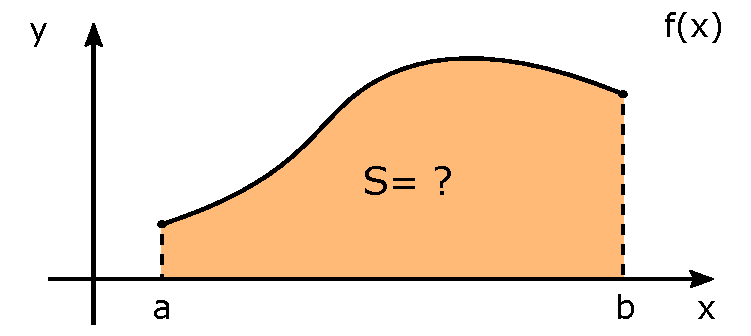
\includegraphics[scale=0.5]{Int.pdf}}
\only<2>{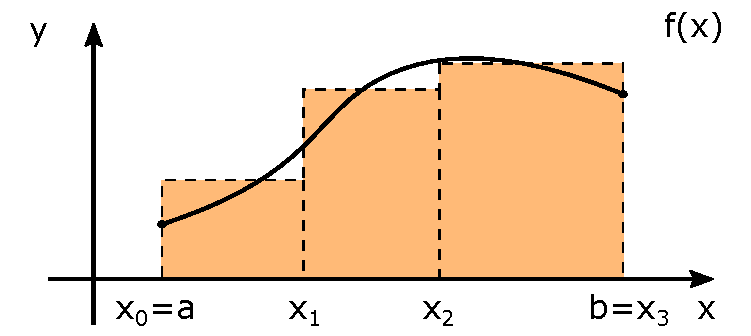
\includegraphics[scale=0.5]{Int2.pdf}}
\end{center}
В качестве приближенного значения площади можно рассмотреть площадь, посчитанную при разбиении криволинейной трапеции на прямоугольники:
$$S\approx \sum_{k=1}^{N} f(\xi_k)(x_{k} - x_{k-1}),$$
где отрезок $[a,b]$ разбит точками $a = x_0<x_1<\ldots<x_{N} = b$ на $N$ частей, $\xi_k$ --- некоторая точка на отрезке $[x_{k-1},x_k]$. Очевидно, что точность подобного приближения будет увеличиваться при увеличении числа точек разбиения. 
\end{block}
\end{frame}

\begin{frame}{Определенный интеграл}
\begin{block}{Определение. Разбиение}
Последовательность точек  $a = x_0<x_1<\ldots<x_{N} = b$ будем называть {\bf разбиением} отрезка $[a,b]$. Введем обозначения
$$\Delta x_k = x_k - x_{x-1},\quad \Delta x  = \max_{k=1,\ldots,N} \Delta x_k.$$
Величину $\Delta x$ называют {\bf параметром разбиения}.
\end{block}
\begin{block}{Определение. Определенный интеграл}
Будим говорить, что функция $f(x)$ {\bf интегрируема} (в смысле Римана) на отрезке $[a,b]$, если существует конечный предел интегральных сумм:
$$S=\lim_{\Delta x\to0} \sum_{k=1}^{N} f(\xi_k)\Delta x_k,$$
для произвольного разбиения и произвольного выбора промежуточных точек $\xi_k\in[x_{k-1},\ x_k]$. Тогда величину $S$ называют {\bf определенным интегралом} от функции $f(x)$ по отрезку $[a,b]$:
$$\int_a^b f(x)dx = S.$$
\end{block}
\end{frame}

\begin{frame}{Определенный интеграл}
\begin{block}{Замечания}
Величину $a$ называют нижним пределом интегрирования, а величину $b$ --- верхним пределом интегрирования.
\vskip1em
В определении интеграла мы потребовали не просто существования предела интегральных сумм, а также его независимости от выбора разбиений отрезка и от выбора промежуточных точек.
\vskip1em
Формально определение интеграла можно расписать следующим образом. Величина $S$ --- значение определенного интеграла от $f(x)$ по отрезку $[a,b]$, если для любого $\varepsilon>0$ существует такое $\delta(\varepsilon)>0$, что справедливо неравенство:
$$\left| S- \sum_{k=1}^{N} f(\xi_k)\Delta x_k \right|<\varepsilon,$$
для любого разбиения $x_i$ и любого выбора точек $\xi_i$ при условии, что параметр разбиения $\Delta x = \max_k\Delta x_k<\delta$.
\vskip1em
Из определения видно, что участки, где $f(x)<0$, дают отрицательный вклад в величину определенного интеграла. В дальнейшем будет видны преимущества такого соглашения.
\end{block}
\end{frame}

\begin{frame}{Интегрируемость функций}
\begin{block}{Предложение}
Интегируемая функция необходимо ограничена.
\end{block}
\vskip-1em
\begin{block}{Доказательство}
Предположим обратное. Пусть $f(x)$ неограничена на отрезке $[a,b]$ (
$\sup |f(x)| = +\infty$).

Тогда она, очевидно, неограничена хотя бы на одном из промежутков разбиения $[x_{k-1},x_{k}]$. Выбирая точку $\xi_k$, можно сделать величину $f(\xi_k)$, а с ней и значение интегральной суммы, сколь угодно большими по модулю.
\end{block}
\vskip-1em
\begin{block}{Определение. Верхние и нижние суммы Дарбу}
Для произвольного разбиения отрезка $[a,b]$ и ограниченной функции $f(x)$ определим:
$$S_{d}  = \sum_{k=1}^N M_k \Delta x_k,\quad s_{d}= \sum_{k=1}^N m_k \Delta x_k,$$
$$\text{где} \qquad M_k = \sup_{x\in[x_{k-1},x_k]} f(x),\qquad m_k = \inf_{x\in[x_{k-1},x_k]} f(x).$$
$S_d$ --- верхняя сумма Дарбу, а $s_d$ --- нижняя сумма Дарбу.
\end{block}
\end{frame}

\begin{frame}{Критерий интегрируемости}
Очевидно, что произвольная интегральная сумма лежит между соответствующими суммами Дарбу.
\begin{block}{Теорема. Критерий интегрируемости}
Функция $f(x)$ интегрируема на отрезке $[a,b]$ тогда и только тогда, когда
$ (S_d - s_d) \to0,$
в независимости от выбора разбиения отрезка, лишь только $\Delta x\to 0$.
\end{block}
\begin{center}
\only<1>{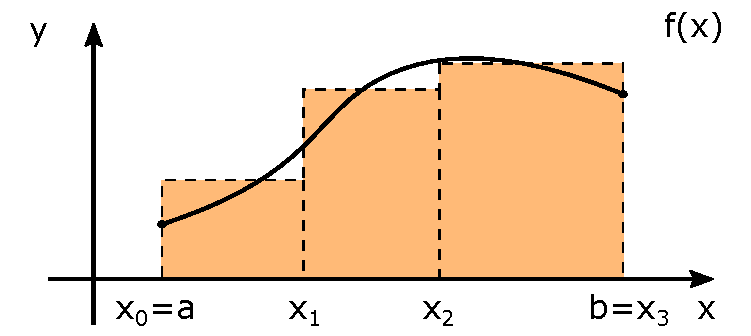
\includegraphics[scale=0.5]{Int2.pdf}}
\only<2>{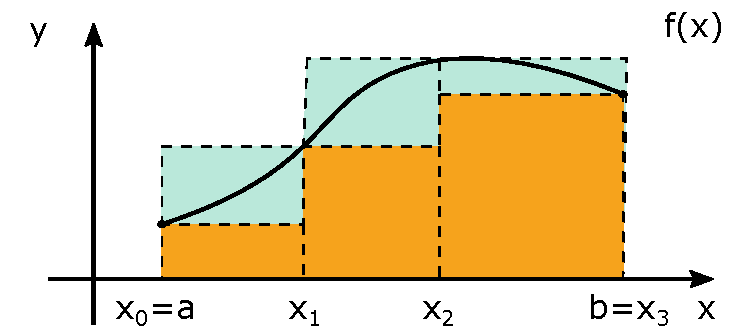
\includegraphics[scale=0.5]{IntD.pdf}}
\end{center}
Приемущество рассмотрения сумм Дарбу заключается в том, что они зависят лишь от разбиения и не зависят от выбора точек $\xi_k$.
\end{frame}

\begin{frame}{Интегрируемость функций}
Строгое определение понятия определенного интеграла позволяет исследовать вопрос о том, какие функции являются интегрируемыми.
\begin{block}{Утверждения}
\begin{enumerate}
\item
Интегрируемая функция необходимо является ограниченной.
\item
Непрерывная функция является интегрируемой.
\item
Ограниченная функция, имеющая конечное число точек разрыва, также является интегрируемой.
\item Если значение интегрируемой функции изменить в одной из точек, то она останется интегрируемой, и значение интеграла не изменится.
\end{enumerate}
\end{block}
\begin{block}{Замечание}
Мы рассматривали интеграл по отрезку $[a,b]$, где $a<b$. По определению положим:
$$\int_a^b f(x)dx= - \int_b^a f(x)dx,\qquad \int_a^a f(x)dx=0.$$ 
В дальнейшем, говоря отрезок  $[b,a]$, где $ b>a$,  будем подразумевать тоже множество $[a,b]$,  но рассмотренное ``в противоположном направлении''.
\end{block}
\end{frame}

\begin{frame}{Линейность интеграла}
\begin{block}{Теорема. Линейность интеграла}
Если функции $f$ и $g$ интегрируемы на отрезке $[a,b]$, то линейная комбинация $A\, f+B\, g$ также интегрируема на $[a,b]$ и
$$\int_a^b \left(A\, f(x)+B\, g(x)\right)dx = A\cdot\int_a^b f(x)dx+B\cdot\int_a^b g(x)dx.$$
\end{block}
\vskip-1em
\begin{block}{Доказательство}
Рассмотрим произвольное разбиение отрезка $[a,b]$. Для доказательства теоремы достаточно перейти к пределу ($\Delta x\to0$) в равенстве интегральных сумм:
$$\sum_{k=1}^N\left( A\, f(\xi_k)+B\, g(\xi_k)\right)\Delta x_k =A\cdot \sum_{k=1}^N f(\xi_k)\Delta x_k+B\cdot\sum_{k=1}^N g(\xi_k)\Delta x_k.$$
\end{block}
\end{frame}

\begin{frame}{Аддитивность интеграла}
\begin{block}{Теорема}
Если функция $f(x)$ интегрируема на отрезке $[a,b]$ и на отрезке $[b,c]$, то она интегрируема на отрезке $[a,c]$ и
$$\int_a^b f(x)dx + \int_b^c f(x) dx = \int_a^c f(x)dx.$$
\end{block}
\vskip-1em
\begin{block}{Доказательство}
Рассмотрим произвольное разбиение отрезка $[a,c]$:
$$a=x_0<x_1<\ldots<x_{r-1}\le b<x_{r}<\ldots<x_N=c.$$
Соответствующие интегральные суммы имеют вид:
$$S_{[a,c]} = \sum_{k=1}^N f(\xi_k) \Delta x_k, \quad
 S_{[a,b]} = \sum_{k=1}^{r-1} f(\xi_k) \Delta x_k+o(1),\quad
 S_{[b,c]} = \sum_{k=r+1}^N f(\xi_k) \Delta x_k+o(1).$$
Переходя к пределу $\Delta x\to0$ в равенстве
$$S_{[a,c]} = S_{[a,b]}+S_{[b,c]}+o(1),$$
получаем свойство аддитивности интеграла, что и требовалось доказать.
\end{block}
\end{frame}

\begin{frame}{Оценки интеграла}
\begin{block}{Теорема. Интегрирование неравенств}
Пусть функции $f$ и $g$ интегрируемы на отрезке $[a,b]$. Тогда
$$f(x)< g(x),\ \forall x\in[a,b]\quad \Rightarrow \int_a^b f(x)dx < \int_a^b g(x)dx,$$
и аналогично в случае нестрогих неравенств.
\end{block}
\begin{block}{Доказательство}
Переходя к пределу в неравенстве для интегральных сумм:
$$ \sum_{k=1}^N f(\xi_k) \Delta x_k\le  \sum_{k=1}^N g(\xi_k) \Delta x_k,$$
получаем соответствующие неравенство для интегралов.
\vskip1em
Для случая строгих неравенств доказательство существенно усложняется, поскольку при переходе к пределу строгие неравенства становятся нестрогими. То, что в этом случае можно все же сохранить строгое неравенство, можно доказать от противного (попробуйте провести подобное доказательство).
\end{block}
\end{frame}

\begin{frame}{Оценки интеграла}
\begin{block}{Теорема. Интегрирование модуля функции}
Пусть функция $f$  интегрируема на отрезке $[a,b]$. Тогда $|f|$ также интегрируем и справедливо неравенство
$$\left| \int_a^b f(x) dx \right| \le \int_a^b |f(x)|dx.$$
\end{block}
\begin{block}{Доказательство}
Если $|f|$ интегрируем, то искомое неравенство следует просто из интегрирования очевидного неравенства
$$-|f(x)|\le f(x)\le |f(x)|.$$
Докажем интегрируемость $|f|$. Рассмотрим произвольное разбиение. Для любых двух точек $x'$ и $x''$ из $[x_{k-1},x_k]$ имеем:
$$|f(x')|-|f(x'')|\le |f(x') - f(x'')|\le M_k - m_k
\text{, где } M_k = \sup_{x\in[x_{k-1},x_k]} f(x),\ m_k = \inf_{x\in[x_{k-1},x_k]} f(x).$$
Следовательно, разность сумм Дарбу для $|f|$ не больше, чем соответствующая разность для $f$, и интегрируемость $|f|$ следует из критерия интегрируемости.
\end{block}
\end{frame}

\begin{frame}{Оценки интеграла}
\begin{block}{Теорема о среднем}
Пусть функция $f$  интегрируема на отрезке $[a,b]$, $m\le f(x)\le M$. Тогда
$$m(b-a)\le\int_a^b f(x) dx\le M(b-a),\quad\text{или}\quad \int_a^b f(x) dx=\mu (b-a),$$
где $m\le \mu \le M$.
\end{block}
\begin{block}{Доказательство}
Данное утверждение следует из интегрирования неравенства $m\le f(x)\le M$ и того, что
$$\int_a^b dx = b-a.$$
\end{block}
\vskip-1em
\begin{block}{Упражнение}
Исходя из определения интеграла, докажите строго, что интеграл от $1$ равен длине отрезка интегрирования (последнее равенство).
\end{block}
\end{frame}

\begin{frame}{Теорема о среднем}
\begin{block}{Следствие}
Если $f$ --- непрерывная функция, то по теореме о промежуточном значении найдется точка $c\in[a,b]$ такая, что
$$\int_a^b f(x) dx = f(c)(b-a).$$
\end{block}
Геометрический смысл последнего утверждения состоит в том, что найдется точка $c$ такая, что площадь криволинейной трапеции совпадает с площадью прямоугольника высоты $f(c)$.
\begin{center}
\only<1>{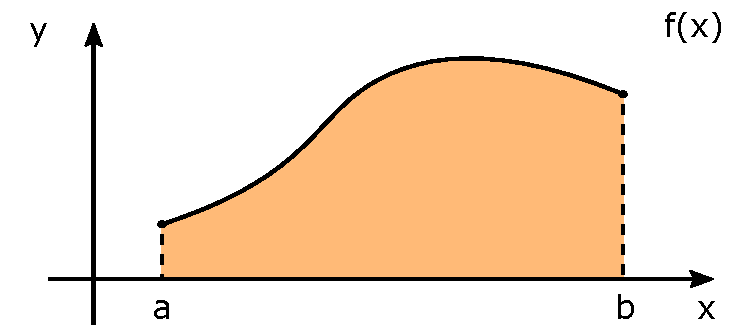
\includegraphics[scale=0.6]{IntM1.pdf}}
\only<2>{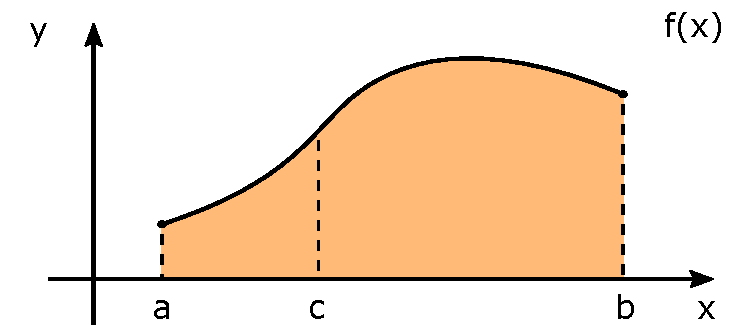
\includegraphics[scale=0.6]{IntM2.pdf}}
\only<3>{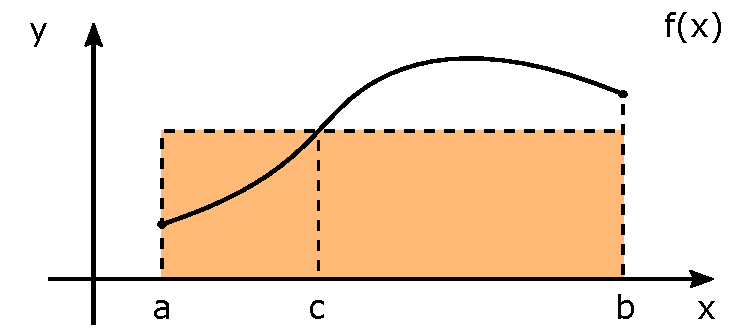
\includegraphics[scale=0.6]{IntM3.pdf}}
\end{center}
\end{frame}

\begin{frame}{Обобщенная теорема о среднем}
\begin{block}{Теорема}
Пусть функции $f$ и $g$ интегрируемы на отрезке $[a,b]$, $m<f(x)<M$, и функция $g$ не меняет знак, то есть $g(x)\le 0$ или $g(x)\ge 0$ для всех $x\in[a,b]$. Тогда
$$\int_a^b f(x)g(x)dx = \mu \int_a^b g(x)dx.$$
Если функция $f(x)$ непрерывна, то существует точка $c\in[a,b]$ такая, что
$$\int_a^b f(x)g(x)dx = f(c) \int_a^b g(x)dx.$$
\end{block}
\begin{block}{Упражнения}
Проверьте, что из обобщенной теоремы о среднем следует обычная теорема о среднем для интеграла.
\vskip0.5em
Докажите интегрируемость произведения интегрируемых функций, используя суммы Дарбу и критерий интегрируемости.
\vskip0.5em
Докажите представленную выше теорему.
\end{block}
\end{frame}

\begin{frame}{Интеграл как функция верхнего предела}
Пусть функция $f$ интегрируема на отрезке $[a,b]$. Тогда она интегрируема и на любом отрезке $[a,x]$, где $x\in[a,b]$.
\vskip1em
Рассмотрим определенный интеграл функции $f$ по отрезку $[a,x]$ как функцию верхнего предела интегрирования
$$\Phi(x) = \int_a^x f(t)dt.$$
Исследуем свойства функции $\Phi(x)$.

\begin{block}{Теорема (Непрерывность интеграла)}
Если $f$ интегрируема на $[a,b]$, то $\Phi$ является непрерывной на этом отрезке.
\end{block}
\begin{block}{Доказательство}
Действительно, применяя свойство аддитивности и теорему о среднем, получаем 
$$\Phi(x+h) - \Phi(x) = \int_a^{x+h}f(t)dt - \int_a^x f(t)dt = \int_x^{x+h} f(t)dt =
\mu h \to 0\quad (h\to0),$$
где $\mu$ --- ограниченная величина, которая зависит от $x$ и от $h$.
\end{block}
Следовательно, при интегрируемости функции ее особые точки ``сглаживаются''.
\end{frame}

\begin{frame}{Интеграл как функция верхнего предела}
\begin{block}{Теорема (Дифференцируемость интеграла)}
Если $f$ интегрируема на $[a,b]$ и непрерывна в точке $x_0\in[a,b]$, то $\Phi$ дифференцируема в $x_0$ и
$$\Phi'(x_0) = f(x_0)\qquad \text{или}\qquad \frac{d}{dx}\Big|_{x_0}\,\int_a^x f(t)dt = f(x_0).$$
\end{block}
\vskip-1em
\begin{block}{Доказательство}
Из непрерывности $f$ в точке $x_0$ следует, что
$$f(x) = f(x_0) + \alpha(x),\quad \alpha(x) = o(x-x_0).$$
Применяя теорему о среднем (следствие) получаем, что
$$\Phi(x_0+h) - \Phi(x_0) = \int_{x_0}^{x_0+h}\left( f(x_0) + \alpha(t) \right)dt = f(x_0) h + \alpha(\xi) h.$$
Поскольку $\xi\in[x_0,x_0+h]$, то $\alpha(\xi) = o(1)$ при $h\to0$. Следовательно,
$$\Phi(x_0+h) - \Phi(x_0) = f(x_0) h + o(h),$$
что и требовалось доказать.
\end{block}
\end{frame}

\begin{frame}{Формула Ньютона--Лейбница}
Последняя теорема является одним из ключевых утверждений интегрального исчисления.
\begin{block}{Следствие. Существование первообразной}
Если $f$ непрерывна на $[a,b]$, то функция $\Phi(x)$ --- определенный интеграл $f$ по отрезку $[a,x]$, является первообразной функции $f$.
\vskip1em
Таким образом, у непрерывной функции всегда существует первообразная.
\end{block}
Пусть $F(x)$ --- некоторая первообразная $f$ на отрезке $[a.b]$. Тогда
$$F(x) = \Phi(x) + C = \int_a^x f(t)dt + C.$$
Подставляя в последнее равенство $x=a$, получаем
$$F(a) = C\quad \Rightarrow \quad F(x) = F(a) + \int_a^x f(t)dt.$$
Следовательно, справедлива теорема.

\begin{block}{Теорема. Формула Ньютона--Лейбница}
Пусть $f$ непрерывна на $[a,b]$, a $F(x)$ --- некоторая первообразная функции $f$. Тогда
$$\int_a^b f(x) dx = F(b) - F(a) = F(x)\Big|_a^b
\qquad \text{или}\qquad
\int_a^b d F(x) = F(b) - F(a).
$$
\end{block}
\end{frame}

\begin{frame}{Формула Ньютона--Лейбница. Следствия}
Таким образом, задача поиска первообразной функции (неопределенный интеграл) и задача поиска площади криволинейной трапеции (определенный интеграл) тесно связаны друг с другом.
\vskip1em
Так, если задача состоит в определении первообразной $F$ для непрерывной функции $f$ на отрезке $[a,b]$, то ответом может служить
$$F(x) = C + \int_a^x f(t)dt, \quad \text{поскольку} \quad \left( C + \int_a^x f(t)dt \right)'=f(x).$$
Наоборот, если известна первообразная $F$ для непрерывной функции $f$, то величину площади криволинейной трапеции можно вычислить, как
$$\int_a^b f(x)dx = F(b) - F(a), \quad \text{поскольку} \quad \int_a^b f(x)dx=\int_a^b dF(x) = F(b) - F(a).$$
Если в формуле Ньютона--Лейбница применить теорему о среднем для интеграла, то получим формулу конечных приращений Лагранжа:
$$F(b) - F(a) = \int_a^b f(x)dx = f(c)(b-a) = F'(c) (b-a).$$
\end{frame}

\begin{frame}{Примеры вычисления определенного интеграла}
Формула Ньютона--Лейбница является одним из основных инструментов вычисления определенного интеграла.
\begin{block}{Примеры}
$$\int_0^{\pi}\sin(x)dx = -\cos x\, \Big|_0^{\pi} = -( \cos \pi - \cos 0) =2.$$
$$\int_1^a \frac{dx}{x} = \ln x \, \Big|_1^a  =\ln a.$$
$$\int_0^1 \frac{dx}{x^2+1} = \arctg x\, \Big|_0^1 = \frac{\pi}{4}.$$
\end{block}
Вспоминая определение для определенного интеграла, выбирая равномерное разбиение отрезка $[0,1]$:
$$x_k = k/n,\quad \xi_k = x_k,$$
получаем, что
$$\frac{\pi}{4} = \int_0^1 \frac{dx}{x^2+1} = \lim_{n\to+\infty} \sum_{k=1}^n \frac{1}{x_k^2+1}\, \frac{1}{n} =
 \lim_{n\to+\infty} n \left( \frac{1}{1^2+n^2}+\frac{1}{2^2+n^2}+\cdots+ \frac{1}{n^2+n^2}\right).$$
 Таким образом, вместо вычисления определенного интеграла как предела, достаточно сложных интегральных сумм, часто наоборот вычисление пределов сложных сумм сводят к вычислению интегралов.
\end{frame}

\begin{frame}{Интегрирование по частям для определенного интеграла}
Для поиска первообразной заданной функции $f$, вычисляя соответствующий неопределенный интеграл, мы выполняли замены переменной и интегрирование по частям. С другой стороны, эти операции удобно проделывать сразу в определенном интеграле.
\begin{block}{Теорема. Интегрирование по частям для определенного интеграла}
Пусть $u(x)$ и $v(x)$ непрерывно дифференцируемые функции на отрезке $[a,b]$. Тогда
$$\int_a^b u(x) v'(x) dx = u(x) v(x)\,\Big|_a^b - \int_a^b u'(x)v(x)dx.$$
\end{block}
\vskip-1em
\begin{block}{Доказательство}
Действительно, применяя формулу Ньютона--Лейбница, получаем
$$ \int_a^b u(x) v'(x) dx +  \int_a^b u'(x)v(x)dx = \int_a^b \left(u(x) v(x)\right)'dx = u(b)v(b) - u(a)v(a) = u(x) v(x)\,\Big|_a^b\,.$$
Остается только перенести один из интегралов в правую часть равенства.
\end{block}
\begin{block}{Пример}
$$\int_0^{\pi/2} x\sin(x)\, dx = - \int_0^{\pi/2} x\,d\cos(x) = - x\cos(x)\Big|_0^{\pi/2} + \int_0^{\pi/2} \cos(x) dx = 0+\sin(x)\Big|_0^{\pi/2} = 1.$$
\end{block}

\end{frame}

\begin{frame}{Замена переменных в определенном интеграле}

\begin{block}{Теорема. Замена переменных в определенном интеграле}
Пусть $f(x)$ --- непрерывная функция на отрезке $[a,b]$. Тогда
$$\int_a^b f(x) dx = \int_{\alpha}^{\beta} f\left(g(t)\right)g'(t)dt,$$
где $g(t)$ --- произвольная функция, удовлетворяющая условиям:
\begin{enumerate}
\item $g(t)$ непрерывно дифференцируемая функция на отрезке $[\alpha,\beta]$, $g\in C^1[\alpha,\beta]$;
\item образ отрезка  $[\alpha,\beta]$ лежит в $[a,b]$, то есть $g(t)\in[a,b]$ при $t\in[\alpha,\beta]$;
\item справедливы граничные условия $g(a) = \alpha$, $g(b) = \beta$.
\end{enumerate}
\end{block}
\vskip-1em
\begin{block}{Доказательство}
Пусть $F(x)$ --- первообразная функции $f$ на отрезке $[a,b]$. Тогда, применяя формулу Ньютона--Лейбница, получаем
$$ \int_{\alpha}^{\beta} f\left(g(t)\right)g'(t)dt = \int_{\alpha}^{\beta}\frac{d}{dt}\left( F\left(g(t)\right)\right)dt = F(g(\beta)) - F(g(\alpha)) = F(b) - F(a) = \int_a^b f(x) dx.$$
\end{block}
Заметим, что второе условие, наложенное на функцию $g$, обеспечивает непрерывность $F(g(t))$, что необходимо для применения формулы Ньютона--Лейбница.
\end{frame}

\begin{frame}{Примеры интегрирования}
Вычислим интеграл
$$ \int_{-a}^a \sqrt{a^2 - x^2} dx = \left\{ x = a \sin(t),\ dx = a \cos(t) dt,\ x=\pm a \ \Rightarrow t = \pm \pi/2 \right\} =$$
$$=
\int_{-\pi/2}^{\pi/2} a^2 \cos^2(t)dt =\frac{a^2}{2} \int_{-\pi/2}^{\pi/2} (1+\cos(2t))dt = \frac{a^2}{2}\left( \pi + \frac{1}{2}\sin(2t)\Big|_{-\pi/2}^{\pi/2}\right)=\frac{1}{2}\pi a^2.$$
Получили ожидаемый результат, поскольку данный интеграл представляет половину площади окружности.
\end{frame}

\begin{frame}{Формула Тейлора}
Запишем формулу Ньютона--Лейбница в виде
$$f(b) - f(a) = \int_a^b f'(x)dx.$$
Интегрируя по частям, получаем:
$$\int_a^b f'(x)dx = - \int_a^b f'(x) d(b-x) = - f'(x)(b-x)\Big|_a^b + \int_a^b f''(x) (b-x) dx \ \Rightarrow$$
$$f(b)-f(a) = f'(a)(b-a) +  \int_a^b f''(x) (b-x) dx.$$
Внесем множитель $(b-x)$ под дифференциал и еще раз проинтегрируем по частям:
$$\int_a^b f''(x) (b-x) dx = - \frac{1}{2} \int_a^b f''(x) d(b-x)^2 =
\frac{f''(a)}{2}(b-a)^2 + \frac{1}{2} \int_a^b f^{(3)}(x)(b-x)^2dx \ \Rightarrow$$
$$f(b) = f(a) + f'(a)(b-a) +  \frac{f''(a)}{2}(b-a)^2 + \frac{1}{2} \int_a^b f^{(3)}(x)(b-x)^2dx.$$
Внеинтегральный член в последней формуле нам хорошо знаком --- это многочлен Тейлора для функции $f$.
\end{frame}

\begin{frame}{Формула Тейлора}
Продолжая интегрирование по частям, мы получаем следующую теорему.
\begin{block}{Теорема. Формула Тейлора с интегральным остаточным членом.}
Пусть функция $f(x)\in C^{n+1}[a,b]$. Тогда
$$f(x) = f(a) + f'(a)(x-a)+\cdots+\frac{f^{(n)}(a)}{n!}(x-a)^n+\frac{1}{n!}\int_a^x f^{(n+1)}(t)(x-t)^n dt,$$
где $x$ --- произвольная точка из $[a,b]$.
\end{block}
Мы уже доказали это утверждение для $n=1$ и $n=2$. 

\begin{block}{Упражнение}
Проведите доказательство данной теоремы методом математической индукции по~$n$.
\end{block}

Таким образом, мы получили новую формулу для остаточного члена в формуле Тейлора. Применяя общую теорему о среднем, получаем
$$r_n(x) = \frac{1}{n!}\int_a^x f^{(n+1)}(t)(x-t)^n dt = 
\frac{ f^{(n+1)}(\xi)}{n!}\int_a^x (x-t)^n dt = \frac{ f^{(n+1)}(\xi)}{(n+1)!}(x-a)^{n+1},$$
то есть формулу Лагранжа для остаточного члена.

\end{frame}

\begin{frame}{Путь в пространстве}
Рассмотрим задачу об определении длины пути, пройденного точкой за определенной промежуток времени.

\begin{block}{Определение. (Путь)}
{\bf Путем} в трехмерном пространстве $\mathbb{R}^3$ называют непрерывное отображение $r(t) = (x(t),\ y(t),\ z(t))$ промежутка времени $t\in[\alpha,\ \beta]$ в трехмерное пространство $\mathbb{R}^3$.
\vskip1em
Точку $A=r(\alpha)$ называют началом пути, а точку $B=r(\beta)$ --- концом пути. Если начало и конец пути совпадают $A=B$, то путь называют {\bf замкнутым}.
\vskip1em
Если отображение $r$ является взаимно-однозначным, то путь называют {\bf простым}. Такой путь не имеет самопересечений.
\end{block}
Аналогично вводится понятие пути в произвольном пространстве, например, на плоскости или на сфере.
\vskip1em
Путь называют {\bf гладким}, если функции $x(t)$, $y(t)$ и $z(t)$ являются гладкими, то есть непрерывно дифференцируемыми любое число раз. Требование существования производных позволяет говорить о скорости движения по пути.
\end{frame}

\begin{frame}{Путь в пространстве}
\begin{block}{Пример}
Рассмотрим верхнюю половину окружности радиуса $R$ на плоскости $(x,y)$. Ее можно представить как траекторию различных путей. Например,
$$r_1(t):\quad x(t) =R \cos(t),\ y(t) = R \sin(t),\ t\in[0,\pi];$$
$$r_2(t):\quad x(t) = t,\ y(t) = \sqrt{R^2-t^2},\ t\in[-R,R].$$
Пути $r_1$ и $r_2$ отличаются параметризацией, хотя и представляют одну и туже траекторию.
\end{block}
\begin{center}
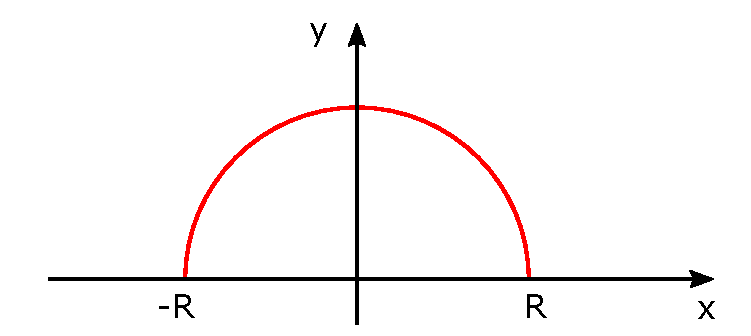
\includegraphics[scale=0.6]{circl.pdf}
\end{center}
\end{frame}

\begin{frame}{Длина пути}
Рассмотрим гладкий путь $r(t)$ на плоскости.
\vskip1em
Естественно под длиной пути понимать предел длин всевозможных ломаных, выписанных в траекторию пути, при стремлении звеньев ломаной к нулю. Длина  ломаной имеет вид:
$$p= \sum_{k=1}^N \left|r(t_k) - r(t_{k-1})\right| = \sum_{k=1}^N \sqrt{\left( x(t_k) - x(t_{k-1})\right)^2+\left(y(t_k) - y(t_{k-1})\right)^2},$$
где $r(t_k) = (x(t_k),\ y(t_k))$ --- точки разбиения траектории пути, соответствующие узлам ломаной. Вынося множитель $\Delta t_k = t_k - t_{k-1}$ из под корня, получим
$$p= \sum_{k=1}^N \sqrt{\left( \frac{x(t_k) - x(t_{k-1})}{ t_k - t_{k-1}}\right)^2+\left(\frac{y(t_k) - y(t_{k-1})}{ t_k - t_{k-1}}\right)^2}\Delta t_k.$$
Несложно доказать, что пределом подобных сумм служит интеграл
$$l=\int_\alpha^\beta \sqrt{(x'(t))^2+(y'(t))^2}dt.$$
Величину $l$ будем называть {\bf длиной пути} $r(t)$. 
\end{frame}

\begin{frame}{Длина пути. Пример}
\begin{block}{Длина окружности}
Рассмотрим параметризацию окружности:
$$x= R \cos(t),\ y=R \sin(t),\ t\in[0,\ 2\pi].$$
Тогда
$$l =\int_\alpha^\beta \sqrt{\dot x^2(t)+\dot y^2(t) }dt = \int_0^{2\pi} \sqrt{ R^2 (-\sin(t))^2+R^2(\cos(t))^2}dt = R\int_0^{2\pi}dt = 2\pi R.$$
\end{block}
\vskip-1em
\begin{block}{Длина графика функции}
Пусть на отрезке $[a,b]$ задана функция $f$. Найдем длину графика функции $f$. Простейшая параметризация имеет вид:
$$x= t,\ y=f(t),\ t\in[a,\ b].$$
Тогда
$$l =\int_a^b \sqrt{1+(f'(t))^2}dt = \int_a^b \sqrt{1+(f'(x))^2}dx.$$
\end{block}
\vskip-1em
\begin{block}{Упражнение}
Найдите длину параболы $y=x^2$ на отрезке $x\in[-1,1]$.
\end{block}
\end{frame}

\begin{frame}{Объем тела вращения}
Рассмотрим задачу об определении объема тела с заданной площадью поперечного сечения $S(x)$, где $x\in[a,b]$.
\vskip1em
Если взять разбиение отрезка $[a,\ b]$:
$$a = x_0< x_1<\ldots <x_n = b,\quad \Delta x_k = x_k - x_{k-1},\quad \Delta x  =\max \Delta x_k,$$
то объем исходного тела можно приблизить суммой объемов цилиндров с сечением $S(x_i)$ и высотой $\Delta x_i$. Соответствующая приближенная формула имеет вид:
$$\sum_{k=1}^n S(x_k)\Delta x_k.$$
Предположим, что функция $S(x)$ непрерывна на $[a,b]$. Тогда, устремляя $\Delta x\to0$, получаем
$$V = \lim_{\Delta x\to0} \sum_{k=1}^n S(x_k)\Delta x_k = \int_a^b S(x) dx.$$

\end{frame}

\begin{frame}{Объем тела вращения}
Важный пример применения предыдущей формулы --- это вычисления объема тела вращения.
\vskip1em
Рассмотрим непрерывную положительную функцию $f(x)$ на отрезке $[a,b]$. Телом вращения графика функции $y = f(x)$ относительно оси абсцисс (ось $x$) называют множество точек
$$M = \left\{ (x,y,z)\in\mathbb{R}^3 \mid y^2+z^2\le f^2(x) \right\}.$$
То есть поперечное сечение тела $M$ плоскостью $x = x_0$ --- это круг радиуса $f(x)$. Площадь этого круга равна $\pi f^2(x)$, а объем соответствующего тела вращения имеет вид
$$V = \pi \int_a^b f^2(x)dx.$$
\begin{center}
\vskip-1em
\only<1>{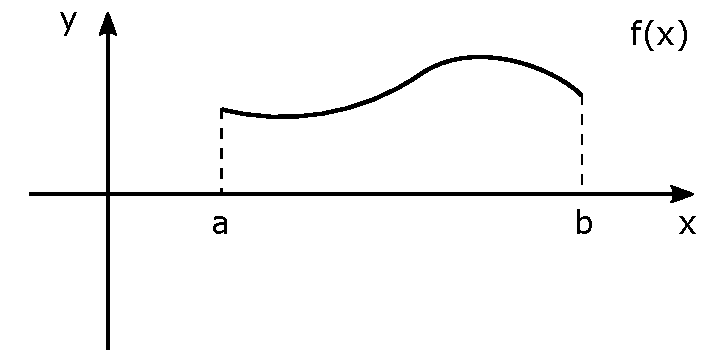
\includegraphics[scale=0.5]{frot.pdf}}
\only<2>{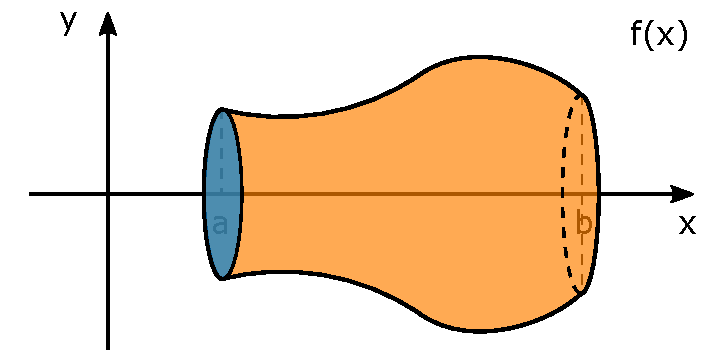
\includegraphics[scale=0.5]{frot2.pdf}}
\end{center}
\end{frame}

\begin{frame}{Несобственный интеграл}
В различных задачах, связанных с интегрированием, часто возникает необходимость вычисления интеграла
$$\int_a^b f(x) dx$$
в более общем случае, чем мы рассматривали ранее. Например, если функция $f(x)$ не является ограниченной на отрезке $[a,b]$ или если один из пределов интегрирования равен бесконечности. Например,
$$\int_0^{+\infty} e^{-x^2}dx\qquad \text{или} \qquad \int_0^1\frac{dx}{\sqrt{1-x^2}}.$$
Здесь мы не можем брать произвольное разбиение, а соответствующий интеграл определять как предел интегральных сумм.
\vskip1em
Простая идея основана на том, что можно вычислить интеграл по конечному отрезку
$$\Phi(A) = \int_a^{A}f(x)dx.$$
Если существует предел $\Phi(A)$ при  $A\to+\infty$, то можно считать:
$$\int_a^{+\infty}f(x)dx = \Phi(+\infty) = \lim_{A\to+\infty}  \int_a^{A}f(x)dx.$$
\end{frame}

\begin{frame}{Несобственный интеграл}
Таким образом мы исключили малую окрестность бесконечно удаленной точки из нашего интеграла и рассмотрели предел интегралов по оставшейся области.
Аналогичным образом поступают и в случае наличия особенностей у функции $f(x)$ в отдельных точках отрезка интегрирования.
 \vskip-0.5em
\begin{block}{Определение. Несобственный интеграл}
Пусть функция $f(x)$ интегрируема на отрезке $[a,A]$ при $\forall A>a$, тогда по определению положим
$$\int_a^{+\infty}f(x)dx = \lim_{A\to+\infty} \int_a^{A}f(x)dx.$$
Соответствующий интеграл называют {\bf несобственным интегралом первого рода}  --- интеграл по бесконечному отрезку.
\vskip1em
Пусть функция $f(x)$ интегрируема на отрезке $[a,\beta]$ при $\forall \beta\in[a,b)$, но не интегрируема на $[a,b]$, тогда по определению положим
$$\int_a^{b}f(x)dx = \lim_{\beta\to b} \int_a^{\beta}f(x)dx.$$
Соответствующий интеграл называют {\bf несобственным интегралом второго рода}  --- интеграл от неограниченной функции.
\end{block}
Если существуют пределы из определения несобственных интегралов, то соответствующие несобственные интегралы называют {\bf сходящимися}.
\end{frame}

\begin{frame}{Несобственный интеграл. Пример}
\begin{block}{Пример. Эталонный несобственный интеграл первого рода.}
Рассмотрим
$$I(\alpha)=\int_1^{+\infty}\frac{dx}{x^\alpha}.$$
По определению, если $\alpha\ne1$:
$$I(\alpha) = \lim_{A\to+\infty} \int_1^A \frac{dx}{x^\alpha} = 
\lim_{A\to+\infty}\left( -\frac{1}{(\alpha-1)x^{\alpha-1}}\Big|_1^A \right) =
\frac{1}{\alpha-1} - \frac{1}{\alpha-1}\lim_{A\to+\infty}\frac{1}{A^{\alpha-1}}\Rightarrow$$
$$I(\alpha)=
\left\{ \begin{array}{ll}
\displaystyle \frac{1}{\alpha-1}& \alpha>1;\\
+\infty & \alpha<1,
\end{array}\right.$$
а в случае $\alpha=1$ получаем:
$$I(1) =  \lim_{A\to+\infty} \int_1^A \frac{dx}{x} = 
\lim_{A\to+\infty}\ln(x)\Big|_1^A = \lim_{A\to+\infty}\ln(A) = +\infty$$
Таким образом, интеграл $I(\alpha)$ сходится при $\alpha>1$ и расходится к $+\infty$ при $\alpha\le1$.
\end{block}
\end{frame}

\begin{frame}{Несобственный интеграл. Пример}
\begin{block}{Пример. Эталонный несобственный интеграл второго рода.}
Рассмотрим
$$J(\alpha)=\int_0^{1}\frac{dx}{x^\alpha}.$$
По определению, если $\alpha\ne1$:
$$J(\alpha) = \lim_{\varepsilon\to+0} \int_\varepsilon^1 \frac{dx}{x^\alpha} = 
\lim_{\varepsilon\to+0} \left(
 -\frac{1}{(\alpha-1)x^{\alpha-1}}\Big|_\varepsilon^1 \right) =
\frac{1}{1-\alpha} - \frac{1}{1-\alpha}\lim_{\varepsilon\to+0}\frac{1}{\varepsilon^{\alpha-1}}\Rightarrow$$
$$J(\alpha)=
\left\{ \begin{array}{ll}
\displaystyle \frac{1}{1-\alpha}& \alpha<1;\\
+\infty & \alpha>1,
\end{array}\right.$$
а в случае $\alpha=1$ получаем:
$$J(1) =  \lim_{\varepsilon\to+0} \int_\varepsilon^1 \frac{dx}{x} = 
\lim_{\varepsilon\to+0}\ln(x)\Big|_\varepsilon^1=- \lim_{\varepsilon\to+0}\ln(\varepsilon) = +\infty$$
Таким образом, интеграл $J(\alpha)$ сходится при $\alpha<1$ и расходится к $+\infty$ при $\alpha\ge1$.
\end{block}
\end{frame}

\begin{frame}{Несобственный интеграл. Пример}
Мы доказали следующие утверждение, которое будет часто применяться в дальнейшем.
\begin{block}{Утверждение}
Интеграл 
$$\int_1^{+\infty}\frac{dx}{x^\alpha}\qquad \text{сходится при $\alpha>1$}$$
и расходится к $+\infty$ при $\alpha\le1$, а интеграл $$\int_0^{1}\frac{dx}{x^\alpha}\qquad \text{сходится при $\alpha<1$}$$
и расходится к $+\infty$ при $\alpha\ge1$.
\end{block}
\begin{block}{Упражнение}
Аналогично, рассмотрите интегралы
$$\int_a^b\frac{dx}{(x-a)^\alpha},\qquad \int_a^b\frac{dx}{(b-x)^\alpha}.$$
\end{block}
\end{frame}

\begin{frame}{Несобственный интеграл. Свойство}
\begin{block}{Теорема}
Пусть функция $f(x)$ интегрируема на отрезке $[a,b]$ в обычном смысле. Тогда 
$$\lim_{z\to b-0} \int_a^z f(x)dx = \int_a^b f(x) dx.$$
Таким образом, несобственный интеграл по отрезку $[a,b]$ совпадает с обычным интегралом в случае интегрируемой функции $f(x)$.
\end{block}
\begin{block}{Доказательство}
Определим функцию
$$F(x) = \int_a^x f(t)dt.$$
Поскольку функция $f(x)$ интегрируема, то $F(x)$ непрерывна. Следовательно,
$$\lim_{x\to b} F(x) = F(b) = \int_a^b f(x)dx,$$
что и требовалось доказать.
\end{block}
\end{frame}

\begin{frame}{Несобственный интеграл. Упражнения}
\begin{block}{Упражнение}
Предположим, что функция $f(x)$ не интегрируема по отрезку $[a,b]$ в обычном смысле, но сходится соответствующий несобственный интеграл. Тогда функция 
$$F(x) = \int_a^x f(t)dt$$
не является непрерывной в точке $x=b$. Каков тип точки разрыва функции $F(x)$ в точке $b$?
\vskip1em
Рассмотрите этот вопрос на примере функции
$$F(x) = \int_{-1}^x\frac{dt}{\sqrt{|t|}}.$$
Вычислите
$$F(x) = \int_{-1}^1\frac{dt}{\sqrt{|t|}}.$$
\end{block}
\end{frame}

\begin{frame}{Несобственный интеграл. Свойства}
Для сходящихся несобственных интегралов справедливы свойства и методы вычисления обычного интеграла.
\vskip 1em
Предположим, что функция $f(x)$ и $g(x)$ интегрируема по отрезку $[a,b]$ в обычном смысле или соответствующие несобственные интегралы сходятся (возможен случай $b=+\infty$ и $a=-\infty$). Тогда справедливы следующие свойства.
\begin{block}{Линейность}
$$\exists\  \int_a^b (A f(x) + B g(x)) dx = A\int_a^b f(x)dx+B\int_a^b g(x)dx.$$
\end{block}
\begin{block}{Аддитивность}
$$\int_a^b f(x)dx = \int_a^c f(x)dx+\int_c^b f(x)dx.$$
\end{block}
\begin{block}{Упражнение}
Проведите полное доказательство данных свойств.
\end{block}
\end{frame}

\begin{frame}{Несобственный интеграл. Замена переменных}
\begin{block}{Теорема о замене переменных в несобственном интеграле}
Пусть сходится несобственный интеграл
$$\int_a^b f(x) dx,$$
где $b$ --- особая точка, то есть $b=\pm\infty$ или $f(x)$ не ограничена в любой окрестности $x=b$. Пусть $x=g(t)$ --- непрерывно дифференцируемая функция на интервале $[\alpha,\beta)$, $g(\alpha)=a$, $g(\beta-0)=b$ и образ интервала $(\alpha,\beta)$ при отображении $g$ лежит в $[a,b]$. Тогда сходится интеграл
$$\int_\alpha^\beta f(g(t))g'(t)dt = \int_a^b f(x)dx.$$
\end{block}
Теорема о замене переменных в сходящемся несобственном интеграле полностью повторяет соответствующее утверждение из теории определенного интеграла, только теперь не требуется дифференцируемости функции $g(t)$ в точке $\beta$. Достаточно выполнения условия
$$g(t)\to b, \quad t\to\beta-0.$$
Из теоремы следует, что в несобственном интеграле также можно вносить функции под дифференциал.
\end{frame}

\begin{frame}{Несобственный интеграл. Пример}
Замена $x=1/t$ позволяет свести исследование несобственного интеграла второго рода к первому роду и наоборот. Например,
$$\int_0^1 \frac{dx}{\sqrt{x}} = \left\{ x=1/t, \ dx = -\frac{dt}{t^2},\ x\to0 \Rightarrow t\to+\infty,\ x=1\Rightarrow t=1\right\} = \int_1^{+\infty} \frac{dt}{t^{3/2}}.$$
Оба интеграла легко вычисляются. Интересно, что оба интеграла являются сходящимися: в интеграле слева $\alpha=1/2<1$, а в интеграле справа $\alpha=3/2>1$.
\begin{block}{Примеры}
Рассмотри несобственный интеграл
$$\int_1^{+\infty} \frac{\cos(1/t)}{t^2}dt = -\int_1^{+\infty} \cos\left(\frac{1}{t}\right) d\frac{1}{t} = -\int_1^0\cos(x)dx = \sin(x)\Big|_0^1 = \sin(1).$$
Заметим, что в этом случае после замены переменных несобственный интеграл превратился в обычный интеграл Римана.
\end{block}
\end{frame}

\begin{frame}{Несобственный интеграл. Интегрирование по частям}
\begin{block}{Теорема об интегрировании по частям в несобственном интеграле}
Пусть функции $f,g\in C^1[a,b)$ и существует
$$\lim_{x\to b-0} f(x)g(x).$$
Тогда несобственные интегралы от $f(x)g'(x)$ и от $f'(x)g(x)$ по $x\in[a,b]$ сходятся или расходятся одновременно. В случае сходимости справедливо равенство:
$$\int_a^b f(x)g'(x)dx = f(x)g(x)\Big|_a^b - \int_a^b f'(x)g(x)dx,$$
где в подстановке подразумевается взятие предела $x\to b$, а не просто подстановка $x=b$.
\end{block}
\begin{block}{Упражнение}
Докажите эту теорему.
\end{block}
\begin{block}{Пример}
$$\int_0^{+\infty}xe^{-x}dx = -\int_0^{+\infty}xde^{-x} =- x e^{-x}\Big|_0^{+\infty} + \int_0^{+\infty}e^{-x}dx = -e^{-x}\Big|_0^{+\infty} = 1.$$
\end{block}
\end{frame}

\begin{frame}{Несобственный интеграл. Пример}
Есть функции, первообразные которых не выражаются через элементарные функции, то есть не известно значение интеграла
$$\int_a^x f(t)dt$$ 
для произвольного $x$, но известно точное значение интегралов для некоторых конкретных значений пределов интегрирования.
\vskip1em
Важным примером этого служит знаменитая формула:
$$\int_{-\infty}^{+\infty}e^{-x^2}dx = \sqrt{\pi}.$$
Доказательство этой формулы будет представлено в дальнейшем.
\vskip1em 
Сейчас вычислим интеграл
$$\int_{-\infty}^{+\infty}x^2e^{-x^2}dx = -\frac{1}{2}\int_{-\infty}^{+\infty} x de^{-x^2} =-\frac{1}{2}x e^{-x^2}\Big|_{-\infty}^{+\infty}+\frac{1}{2}\int_{-\infty}^{+\infty} e^{-x^2}dx = 0+\frac{1}{2}\sqrt{\pi}=\frac{\sqrt{\pi}}{2}.$$
\end{frame}

\begin{frame}{Несобственный интеграл. Критерий Коши}
Пусть рассматривается несобственный интеграл, который не удается вычислить. Тогда важно исследовать вопрос о сходимости соответствующего интеграла. Сильно облегчают эту задачу следующие признаки сходимости.
\vskip1em
Поскольку исследование произвольного несобственного интеграла всегда можно свести к интегралу
$$\int_a^{+\infty}f(x)dx,$$
мы будем рассматривать именно этот интеграл.
\begin{block}{Теорема. Критерий Коши.}
Для сходимости несобственного интеграла
$$\int_a^{+\infty}f(x)dx$$
необходимо и достаточно, что бы
$$\forall \varepsilon>0\ \exists B=B(\varepsilon)>a:\quad b1, b2>B\ \Rightarrow \left| \int_{b_1}^{b_2} f(x)dx \right|<\varepsilon.$$
\end{block}
Данная теорема является прямым следствием критерия Коши существования предела (свойство фундаментальности).
\end{frame}

\begin{frame}{Несобственный интеграл. Абсолютная и условная сходимость}
\begin{block}{Определение}
Рассмотрим несобственный интеграл
$$\int_a^{+\infty}f(x)dx.$$
Говорят, что он сходится {\bf абсолютно}, если сходится интеграл
$$\int_a^{+\infty}|f(x)|dx.$$
Если исходный интеграл сходится, но абсолютной сходимости нет, то говорят, что интеграл сходится {\bf условно}.
\end{block}
Поскольку интеграл от модуля $|f(x)|$ может расходится только к $+\infty$, то условие абсолютной и условной сходимости часто записывают так:
$$\int_a^{+\infty}f(x)dx\ \text{ --- сходится абсолютно}\quad \Leftrightarrow \quad \int_a^{+\infty}|f(x)|dx<+\infty.$$
$$\int_a^{+\infty}f(x)dx\ \text{ --- сходится условно}\quad \Leftrightarrow \quad \exists\int_a^{+\infty}f(x)dx,\ \int_a^{+\infty}|f(x)|dx=+\infty.$$
\end{frame}

\begin{frame}{Несобственный интеграл.  Абсолютная и условная сходимость}

\begin{block}{Теорема}
Из абсолютной сходимости следует сходимость соответствующего интеграла.
\end{block}
\begin{block}{Доказательство}
Пусть сходится интеграл
$$\int_a^{+\infty}|f(x)|dx.$$
Тогда по критерию Коши
$$\forall \varepsilon>0\ \exists B=B(\varepsilon)>a:\quad B\le b1\le  b2\ \Rightarrow  \int_{b_1}^{b_2} |f(x)|dx <\varepsilon.$$
По теореме о сравнении интегралов:
$$\left| \int_{b_1}^{b_2} f(x)dx \right|\le \int_{b_1}^{b_2} |f(x)|dx\le \varepsilon.$$
Следовательно, по критерию Коши, сходится интеграл 
$$\int_a^{+\infty}f(x)dx.$$
\end{block}
\end{frame}

\begin{frame}{Несобственный интеграл. Теорема сравнения}
\begin{block}{Теорема о сравнении}
Пусть 
$$0\le f(x) \le g(x).$$
Тогда из сходимости интеграла
$$\int_a^{+\infty} g(x)dx$$
следует сходимость интеграла
$$\int_a^{+\infty} f(x)dx.$$
В этом случае,
$$\int_a^{+\infty} f(x)dx\le \int_a^{+\infty} g(x)dx.$$
С другой стороны, из расходимости интеграла от $f$ следует расходимость интеграла от $g$.
\end{block}
\begin{block}{Доказательство}
Утверждения теоремы следуют из теоремы Вейерштрасса о монотонной сходимости и теорем о предельных переходах в неравенствах.
\end{block}
\end{frame}

\begin{frame}{Несобственный интеграл. Теорема сравнения}
\begin{block}{Примеры}
Рассмотрим
$$I = \int_{\pi/2}^{+\infty} \frac{\sin(x)}{x^2}dx.$$
Очевидно, справедливо неравенство:
$$\left| \frac{\sin(x)}{x^2} \right| \le \frac{1}{x^2},$$
и сходится интеграл
$$\int_{\pi/2}^{+\infty} \frac{dx}{x^2}.$$
Следовательно, по теореме сравнения сходится интеграл
$$\int_{\pi/2}^{+\infty}\frac{|\sin(x)|}{x^2}dx.$$
Таким образом, интеграл $I$ сходится абсолютно, а следовательно, сходится. 
$$I = 0.1646191209280126922979289458759296116305\ldots$$
\end{block}
\end{frame}

\begin{frame}{Несобственный интеграл. Абсолютная и условная сходимость}
\begin{block}{Примеры}
Рассмотрим 
$$\int_{\pi/2}^{+\infty} \frac{\sin(x)}{x^a}dx, \quad a>0.$$
Поступая как и в предыдущем случае, несложно установить, что интеграл $J$ сходится абсолютно при $a>1$, поскольку при $a>1$ сходится интеграл
$$\int_{\pi/2}^{+\infty} \frac{dx}{x^a}.$$
Рассмотрим $0<a\le 1$. Тогда интегрируя по частям, получаем, что
$$ \int_{\pi/2}^{+\infty} \frac{\sin(x)}{x^a}dx = -\int_{\pi/2}^{+\infty} \frac{d \cos(x)}{x^a} = -\frac{\cos(x)}{x^a}\Big|_{\pi/2}^{+\infty} +\int_{\pi/2}^{+\infty} \cos(x)\,d\frac{1}{x^a} =
- a \int_{\pi/2}^{+\infty} \frac{\cos(x)}{x^{a+1}}dx.$$
Из сходимости интеграла в правой части этого равенства и по теореме об интегрировании по частям для несобственного интеграла следует, что исходный интеграл сходится.
\end{block}
\end{frame}

\begin{frame}{Несобственный интеграл. Абсолютная и условная сходимость}
\begin{block}{Примеры}
Исследуем вопрос об абсолютной сходимости интеграла
$$\int_{\pi/2}^{+\infty} \frac{\sin(x)}{x^a}dx, \quad 0<a\le 1.$$
Рассмотрим
$$\int_{\pi/2}^{+\infty} \frac{|\sin(x)|}{x^a}dx.$$
Справедливо неравенство:
$$0\le |\sin(x)|\le 1\quad \Rightarrow \quad |\sin(x)|\ge \sin^2(x).$$
Следовательно, по теореме сравнения:
$$\int_{\pi/2}^{A} \frac{|\sin(x)|}{x^a}dx\ge \int_{\pi/2}^{A} \frac{\sin^2(x)}{x^a}dx =\frac{1}{2} \int_{\pi/2}^{A} \frac{dx}{x^a} - \frac{1}{2}\int_{\pi/2}^A \frac{\cos(2x)}{x^a}dx.$$
Переходя к пределу при $A\to+\infty$, получаем расходимость интеграла от $\displaystyle \frac{|sin(x)|}{x^a}$. Таким образом, интеграл от $\displaystyle \frac{\sin(x)}{x^a}$ сходится лишь условно при $0<a\le1$.
\end{block}
\end{frame}

\begin{frame}{Несобственный интеграл. Абсолютная и условная сходимость}
\begin{block}{Примеры}
Рассмотрим
$$\int_1^{+\infty} \cos(x^3)dx.$$
Сделаем замену $x^3=t$. Тогда
$$\int_1^{+\infty} \cos(x^3)dx = \int_{1}^{+\infty} \cos(t)dt^{1/3} =  \frac{1}{3}\int_{1}^{+\infty} \cos(t) t^{-2/3}dt.$$
Следовательно, рассматриваемый интеграл сходится, но не является абсолютно сходящимся.
\end{block}
Таким образом, несобственный интеграл
$$\int_1^{+\infty} f(x)dx$$
может сходится, даже если $f(x)\not\to 0$ при $x\to+\infty$. 
\end{frame}

\begin{frame}{Несобственный интеграл. Асимптотическое сравнение}
При исследовании несобственного интеграла на сходимость существенную роль играет только поведение подынтегральной функции $f(x)$ при больших $x$.
\begin{block}{Теорема}
Пусть $f$ и $g$ интегрируемы на отрезке $[a,x]$, для любого $x\ge a$, и
$$f(x) \sim g(x),\quad x\to+\infty.$$
Тогда интегралы
$$\int_a^{+\infty} f(x) dx,\qquad \int_a^{+\infty}g(x)dx$$
сходятся или расходятся одновременно. 
\end{block}
\begin{block}{Доказательство}
Из асимптотической эквивалентности $f$ и $g$ следует, что
$$\lim_{x\to+\infty} \frac{f(x)}{g(x)} = 1 \quad \Rightarrow \quad 
\frac{1}{2}g(x)<f(x)<2g(x), \quad \forall x>x_0.$$
Остается лишь применить теорему сравнения и учесть, что интеграл от $g(x)$ сходится тогда и только тогда, когда сходится интеграл от $2 g(x)$ или от $g(x)/2$.
\end{block}
\end{frame}

\begin{frame}{Несобственный интеграл. Асимптотическое сравнение}
\begin{block}{Примеры}
Рассмотрим
$$\int_0^{+\infty}\frac{dx}{1+x^2}.$$
Поскольку
$$\frac{1}{1+x^2} \sim \frac{1}{x^2},\quad  x\to+\infty,$$
то рассматриваемый интеграл сходится.
\vskip1em
Несложно вычислить,
$$\int_0^{+\infty}\frac{dx}{1+x^2} = \arctg(x)\Big|_0^{+\infty} = \frac{\pi}{2}.$$
\end{block}
\end{frame}

\begin{frame}{Несобственный интеграл. Асимптотическое сравнение}
\begin{block}{Примеры}
Рассмотрим интеграл
$$\int_0^{1}\frac{e^x dx}{\sqrt{1-x^2}}.$$
Это несобственный интеграл второго рода с особой точкой $x=1$. Поскольку
$$\frac{e^x}{\sqrt{1-x^2}} \sim \frac{e}{\sqrt{2(1-x)}}, \qquad (x\to 1),$$
и сходится интеграл
$$\int_0^1\frac{dx}{(1-x)^{1/2}},$$
то исходный интеграл также сходится.
\end{block}
\begin{block}{Упражнение}
Исследуйте на сходимость интеграл
$$\int_0^1\ln\sin(x)\ dx.$$
\end{block}
\end{frame}

\begin{frame}{Несобственный интеграл. Асимптотическое сравнение}
Теорему сравнения для несобственных интегралов можно сформулировать следующем образом. Из сходимости интеграла от $g(x)$ следует сходимость интеграла от $f(x)$, если для всех достаточно больших $x$ справедливо неравенство
$$|f(x)|\le const\cdot g(x),$$
где $const$ --- некоторая константа.
\vskip1em
Подобные условия очень часто возникают в различных разделах математики и ее приложениях. Используют следующие обозначения.
\begin{block}{Определение ``О-большое''}
Будем говорить, что $f(x) = O(g(x))$ при $x\to a$, где $a$ --- число или символ $\pm\infty$, если существует проколотая окрестность $U$ точки $x=a$ и константа $C>0$ такие, что
$$|f(x)|\le C\, g(x),\quad \forall x\in U.$$
В этом случае говорят, что $f(x)$ имеет асимптотический порядок при $x\to a$ {\bf не больший}, чем порядок $g(x)$. 
\vskip1em
Если $f(x)=O(g(x))$ и $g(x) = O(f(x))$, то говорят, что $f$ и $g$ имеют один порядок при~$x\to a$.
\end{block}
\end{frame}

\begin{frame}{Несобственный интеграл. Асимптотическое сравнение}
\begin{block}{Теорема}
Пусть 
$$f(x) = O(g(x)), \quad x\to+\infty.$$
Тогда из сходимости интеграла
$$\int_a^{+\infty}g(x)dx,$$
следует сходимость интеграла
$$\int_a^{+\infty}f(x)dx.$$ 
Если функции $f$ и $g$ одного порядка при $x\to+\infty$, то интегралы от $f$ и $g$ сходятся или расходятся одновременно.
\end{block}
\vskip-0.5em
\begin{block}{Доказательство}
$$f(x) = O(g(x)), \quad x\to+\infty \quad \Rightarrow \quad |f(x)|\le C\cdot  g(x), \quad x>x_0.$$
Следовательно, по теореме сравнения сходится интеграл
$$\int_{x_0}^{+\infty} |f(x)|dx,$$
а следовательно, и интеграл от $f(x)$ на интервале $(a,+\infty)$.
\end{block}
\end{frame}

\begin{frame}{``О-большое''}
Приведем основные свойства символа ``О-большое''
\begin{enumerate}
\item Если символ $O$-большое возникает несколько раз в одной формуле, то считают, что каждый раз он представляет одну из функций из соответствующего класса.
\item Справедливы равенства:
\begin{align*}
&O(f) = f(x)\cdot O(1),\\
&O(f) \pm O(f) = O(f),\\
&2 O(f) = O(f),\\
&O(f)+o(f) = O(f),\\
&const \cdot f= O(f),\\
&O(O(f)) = O(f),\\
&O(f)\cdot O(g) = O(f\cdot g).
\end{align*}
\item Остаточный член в формуле Тейлора:
$$f(x) = f(x_0) + \frac{f'(x_0)}{1!}(x-x_0)+\cdots+\frac{f^{(n)}(x_0)}{n!}(x-x_0)^n+r_{n}(x),$$
можно записать, как
$$r_n(x) = \frac{f^{(n+1)}(\xi)}{(n+1)!}(x-x_0)^{n+1} = O(x-x_0)^{n+1}.$$
\end{enumerate}
\end{frame}


\end{document}